\documentclass[12pt,a4paper]{article}

% --- Dil ve sayfa ---
\usepackage[turkish]{babel}
\shorthandoff{=:!} % babel aktif karakter fix
\usepackage{geometry}
\geometry{margin=2.5cm}
\usepackage{setspace}
\onehalfspacing

% --- FONT (Times New Roman) ---
\usepackage{fontspec}
\setmainfont{Times New Roman}

% --- Matematik ---
\usepackage{amsmath,amssymb}
\usepackage{siunitx}

% --- Tablo ve şekiller ---
\usepackage{graphicx}
\usepackage{booktabs}
\usepackage{array}
\usepackage{float}

% --- Linkler ---
\usepackage{hyperref}
\hypersetup{
  colorlinks=true,
  linkcolor=black,
  citecolor=black,
  urlcolor=black
}
\begin{document}
\begin{titlepage}

\begin{center}
\textbf{İSTANBUL TEKNİK ÜNİVERSİTESİ}\\[1em]
\textbf{Bartın Limanı Öz Tüketim Amaçlı}\\
\textbf{Fotovoltaik (PV) Güneş Enerjisi Santrali}\\
\textbf{Teknik, Ekonomik ve Akademik Analizi}
\end{center}

\vfill

\begin{center}
Seyit Efe Sertkaya\\
\small Öğrenci No: 090220704\\
\textbf{Güz Dönemi 2025}
\end{center}

\end{titlepage}



\newpage
\begin{abstract}
Bu çalışmada İTÜ FIZ443 dersi bünyesinde Bartın Limanı için öz tüketim amaçlı bir fotovoltaik (PV) güneş enerjisi santralinin teknik ve ekonomik fizibilitesi incelenmiştir.
Güneş ışınım verileri NASA POWER veri tabanından alınmış, panel düzlemine gelen ışınım hesaplanmış ve yıllık enerji üretimi tahmin edilmiştir.
Kurulu güç, Bartın Limanı 2011 fizibilite raporunda verilen elektrik tüketimi esas alınarak belirlenmiştir.
Ekonomik analiz kapsamında CAPEX, OPEX, EBITDA, EBIT, NPV ve IRR ayrıntılı olarak hesaplanmıştır.
\end{abstract}

\section{Giriş}
Liman işletmeleri; yük taşıma ekipmanları, aydınlatma sistemleri, idari binalar ve yardımcı tesisler nedeniyle yüksek ve sürekli elektrik tüketimine sahiptir.
Artan enerji maliyetleri ve çevresel kaygılar doğrultusunda, limanlarda öz tüketim amaçlı PV sistemlerin kurulması hem ekonomik hem çevresel açıdan önemli avantajlar sunar.

\section{Veri Kaynakları}
\begin{itemize}
\item NASA POWER Data Access Viewer -- Aylık GHI (ALLSKY\_SFC\_SW\_DWN) verileri.
\item Bartın Konteyner Limanı Fizibilite Raporu (2011) -- Yıllık elektrik tüketimi ve tüketim model varsayımları.
\item Canadian Solar TOPBiHiKu7 (620--650 W) -- Modül teknik özellikleri (hesaplarda 630 Wp alınmıştır).
\end{itemize}

\section{Güneş Enerjisi Potansiyeli Analizi}
NASA POWER'dan alınan aylık GHI (yatay düzlem) değerleri, PV modüllerinin $\beta=30^{\circ}$ eğim ve güney yönelim (azimut $180^{\circ}$) koşulu için panel düzlemine (POA) dönüştürülmüştür.

\subsection{\texorpdfstring{GHI $\rightarrow$ POA dönüşümü}{GHI -> POA dönüşümü}}
Toplam panel düzlemi ışınımı (POA) şu şekilde modellenmiştir:
\begin{equation}
H_{\mathrm{POA}} = H_b R_b + H_d \frac{1+\cos\beta}{2} + H\,\rho_g\,\frac{1-\cos\beta}{2},
\end{equation}
burada $H$ GHI, $H_b$ direkt bileşen, $H_d$ difüz bileşen, $R_b$ geometrik dönüşüm katsayısı ve $\rho_g$ yer yansıtırlığıdır (bu çalışmada $\rho_g=0.20$ alınmıştır).

\begin{figure}[H]
\centering
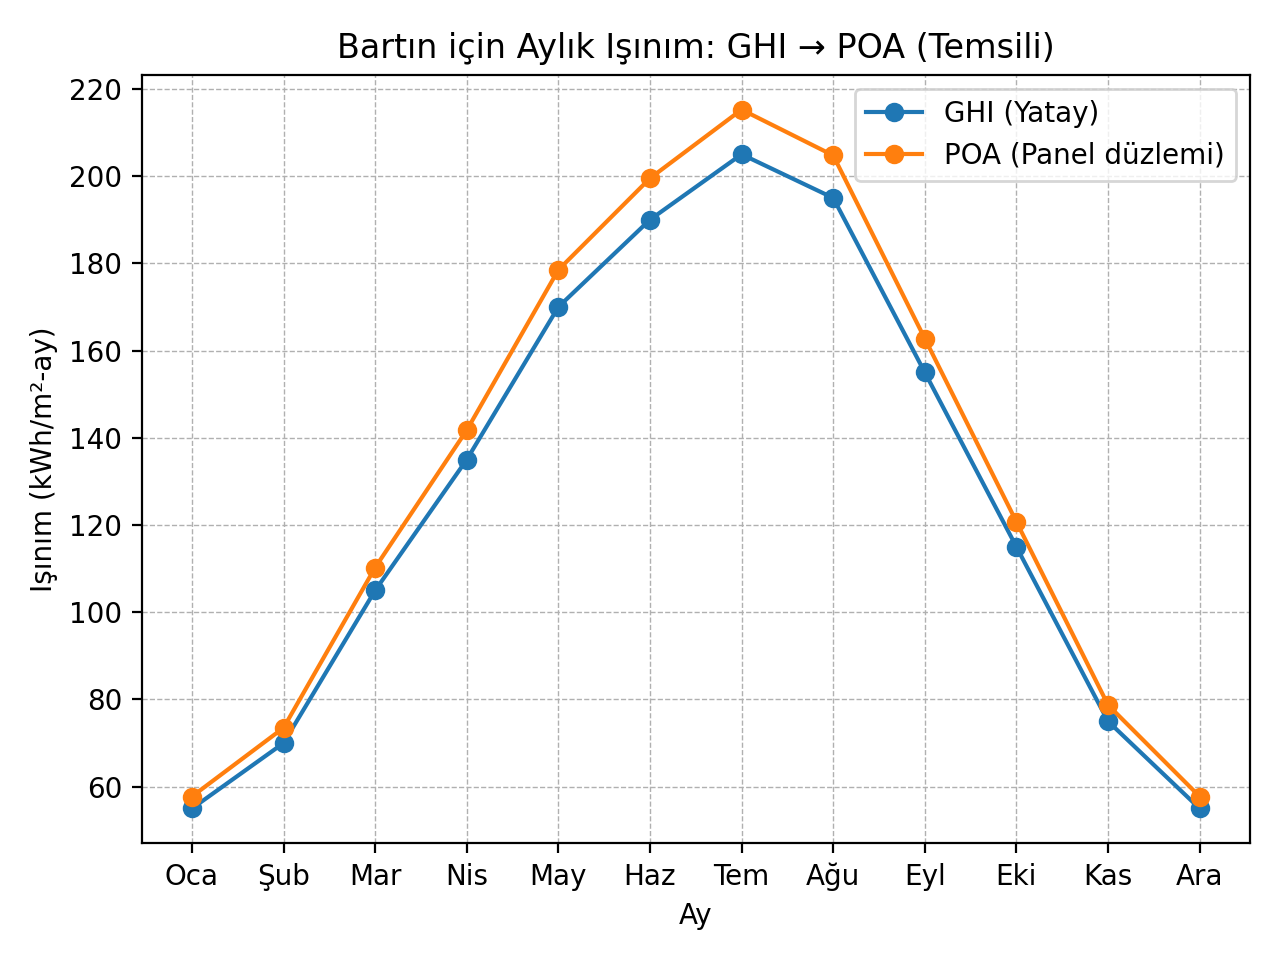
\includegraphics[width=\linewidth]{ghi_poa_bartin.png}
\caption{Bartın için aylık GHI ve 30$^\circ$ güney yönelimli POA karşılaştırması.}
\end{figure}

\section{PV Sistem Tasarımı}
\subsection{Modül seçimi}
Seçilen modül sınıfı: Canadian Solar TOPBiHiKu7 (N-type bifacial TOPCon).
Hesaplamalarda modül gücü $P_{\text{panel}}=\SI{630}{Wp}$ alınmıştır.

\subsection{Performans oranı (PR)}
Sıcaklık, inverter, kablo, mismatch, kirlenme ve kullanılabilirlik kayıpları tek parametrede toplanarak PR $\approx 0.80$ alınmıştır.

\section{Tüketim Tabanlı PV Boyutlandırma}
Bartın Limanı 2011 fizibilite raporunda yıllık elektrik tüketimi yaklaşık $E_{\text{tam}}=\SI{4e6}{kWh/yıl}$ olarak verilmiştir.
Tüketimin \%10'unun sabit, \%90'ının kapasite kullanım oranına (KKO) bağlı olduğu kabul edilerek:
\begin{equation}
E_{\text{yıl}} = E_{\text{tam}} \left(0.10 + 0.90 \times \mathrm{KKO}\right).
\end{equation}

Bartın için özgül üretim (30$^\circ$ güney, PR=0.80) yaklaşık $Y_f=\SI{1279}{kWh/kWp\cdot yıl}$ alınmıştır.
Gerekli DC kurulu güç:
\begin{equation}
P_{\text{DC}}(\text{kWp}) = \frac{E_{\text{yıl}}(\text{kWh/yıl})}{Y_f(\text{kWh/kWp\cdot yıl})}.
\end{equation}

\begin{table}[H]
\centering
\caption{Tüketim tabanlı boyutlandırma (630 Wp modül).}
\begin{tabular}{cccc}
\toprule
KKO (\%) & Tüketim (GWh/yıl) & Kurulu Güç (MWp) & Panel Sayısı \\
\midrule
50  & 2.20 & 1.72 & 2,731 \\
70  & 2.92 & 2.28 & 3,624 \\
100 & 4.00 & 3.13 & 4,965 \\
\bottomrule
\end{tabular}
\end{table}

Öz tüketim yaklaşımı için referans senaryo olarak KKO=\%70 durumu ele alınmış ve kurulu güç $P_{\text{kurulu}}\approx \SI{2.3}{MWp}$ kabul edilmiştir.

\section{Yıllık Enerji Üretim Tahmini}
Yıllık PV üretimi:
\begin{equation}
E_{\text{PV}} \approx P_{\text{kurulu}}\,(\mathrm{kWp})
\times Y_f\,(\mathrm{kWh\,kWp^{-1}\,yıl^{-1}})
\end{equation}

$\SI{2.3}{MWp}$ için:
\begin{equation}
E_{\text{PV}} \approx 2300 \times 1279 \approx \SI{2.94}{GWh/yıl}.
\end{equation}

\begin{figure}[H]
\centering
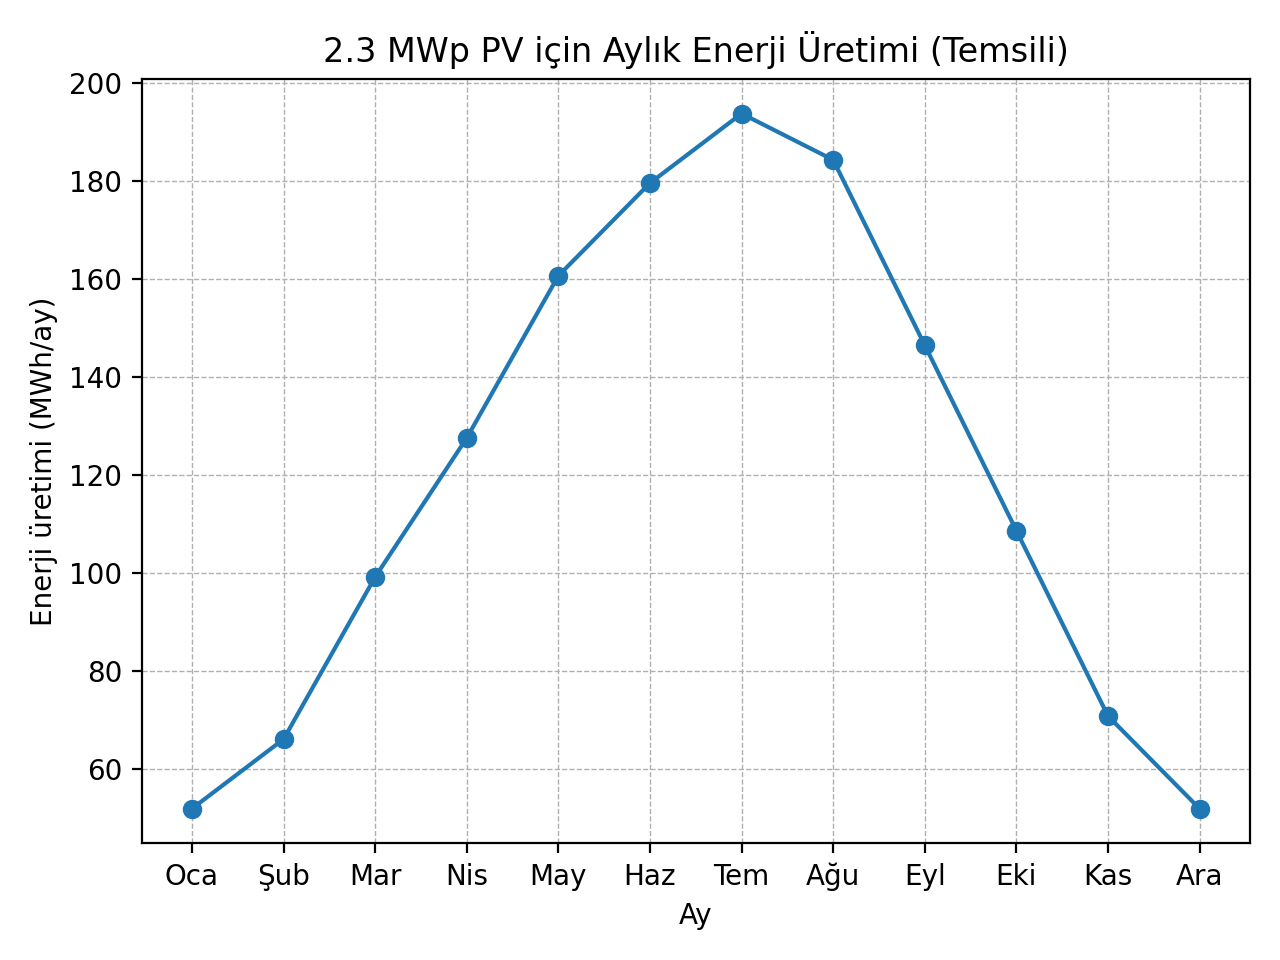
\includegraphics[width=\linewidth]{monthly_energy_23MWp.png}
\caption{$\SI{2.3}{MWp}$ kurulu güç için aylık PV enerji üretimi.}
\end{figure}

\begin{figure}[H]
\centering
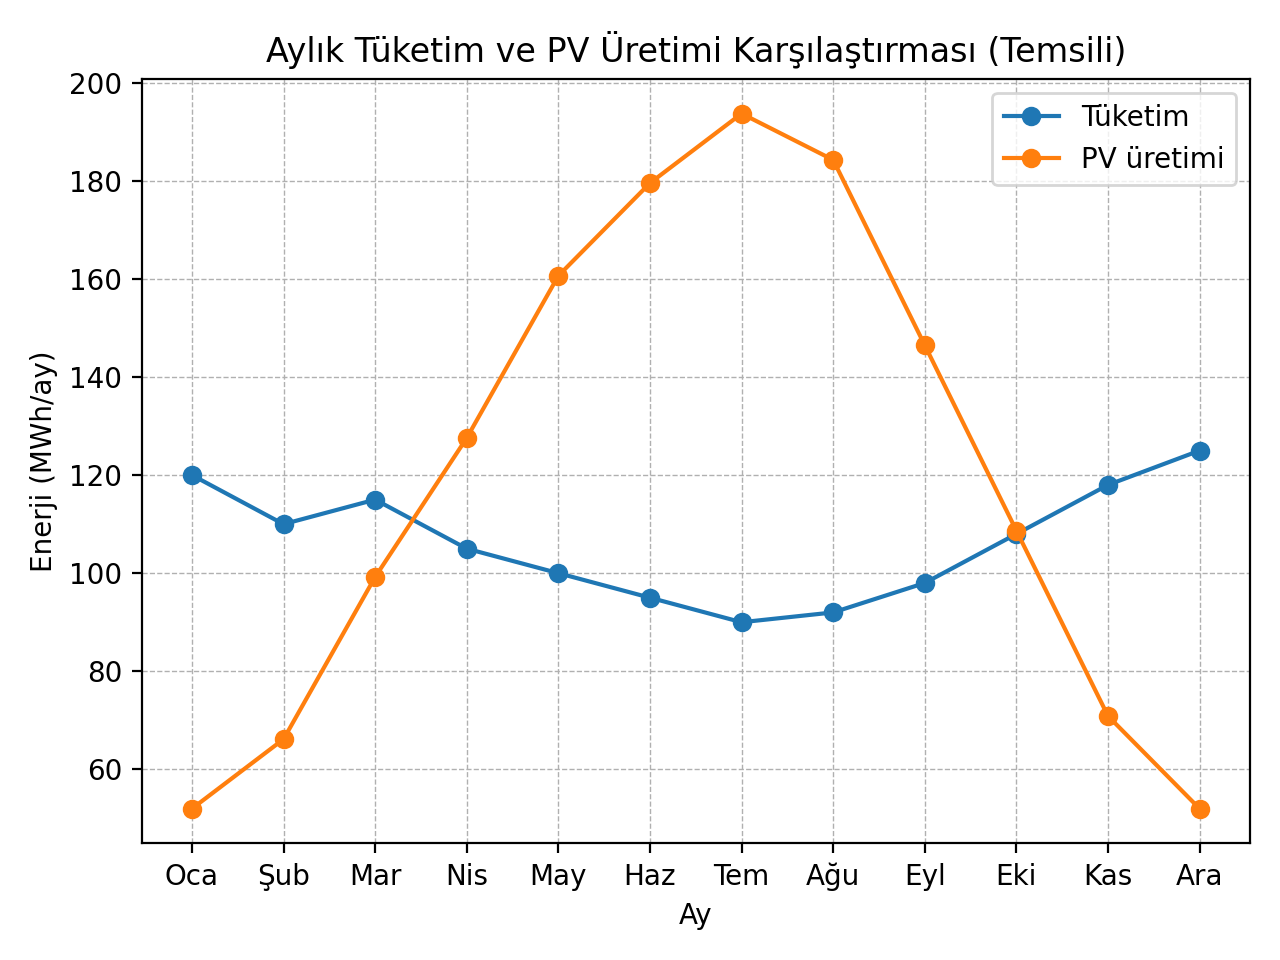
\includegraphics[width=\linewidth]{consumption_vs_pv.png}
\caption{Aylık tüketim (ortalama) ile PV üretiminin karşılaştırılması.}
\end{figure}

\section{Ekonomik Analiz (Öz Tüketim)}
Bu bölümde PV üretiminin geliri, öz tüketim sayesinde \textbf{şebekeden satın alınmayan enerji} olarak modellenmiştir.

\subsection{Gelir (tasarruf) modeli}
Yıllık brüt tasarruf:
\begin{equation}
S_{\text{yıl}} = E_{\text{PV}} \times p_e
\end{equation}
Burada $p_e$ elektrik birim fiyatıdır (TL/kWh).

\subsection{Parametreler ve varsayımlar}
Referans senaryoda kullanılan ana parametreler Tablo~\ref{tab:eco_params}'te verilmiştir.

\begin{table}[H]
\centering
\caption{Ekonomik analiz parametreleri (referans senaryo).}
\label{tab:eco_params}
\begin{tabular}{p{5cm} p{5cm} p{4cm}}
\toprule
Parametre & Tanım & Değer \\
\midrule
$P_{\text{kurulu}}$ & DC kurulu güç & $\SI{2300}{kWp}$ \\
$Y_f$ & Özgül üretim & $\SI{1279}{kWh/kWp\cdot yıl}$ \\
$E_{\text{PV}}$ & Yıllık PV üretimi & $\SI{2.94}{GWh/yıl}$ \\
$p_e$ & Elektrik birim fiyatı & $\SI{4.35}{TL/kWh}$ \\
$c_{\text{capex}}$ & CAPEX birim & $\SI{700}{USD/kW}$ \\
Kur & USD/TL & 42.8 \\
$f_{\text{opex}}$ & OPEX oranı & \%1.5 CAPEX \\
$N$ & Proje ömrü & 12 yıl \\
$r$ & İskonto oranı & \%10 \\
$n_D$ & Amortisman süresi & 10 yıl \\
\%8 CAPEX & İnverter yenileme & Yıl 10 \\
\bottomrule
\end{tabular}
\end{table}

\subsection{CAPEX, OPEX, EBITDA ve EBIT (adım adım)}
Toplam CAPEX:
\begin{equation}
\mathrm{CAPEX}_{\text{TL}} = P_{\text{kurulu}}(\text{kW}) \times c_{\text{capex}}(\text{USD/kW}) \times (\text{USD/TL})
\end{equation}
Yıllık OPEX:
\begin{equation}
\mathrm{OPEX}_{\text{yıl}} = f_{\text{opex}} \times \mathrm{CAPEX}_{\text{TL}}
\end{equation}
EBITDA:
\begin{equation}
\mathrm{EBITDA} = S_{\text{yıl}} - \mathrm{OPEX}_{\text{yıl}}
\end{equation}
Doğrusal amortisman:
\begin{equation}
D = \frac{\mathrm{CAPEX}_{\text{TL}}}{n_D}
\end{equation}
EBIT:
\begin{equation}
\mathrm{EBIT} = \mathrm{EBITDA} - D
\end{equation}

\subsection{Nakit akışı, NPV ve IRR}
Nakit akışı:
\begin{align}
\mathrm{CF}_0 &= -\mathrm{CAPEX}_{\text{TL}} \\
\mathrm{CF}_t &= \mathrm{EBITDA} - \mathrm{Repl}_t \qquad (t=1,\dots,N)
\end{align}
Bu çalışmada $\mathrm{Repl}_{10}=0.08\times \mathrm{CAPEX}_{\text{TL}}$ inverter yenilemesi olarak eklenmiştir.

Net Bugünkü Değer (NPV):
\begin{equation}
\mathrm{NPV} = \sum_{t=0}^{N} \frac{\mathrm{CF}_t}{(1+r)^t}
\end{equation}
IRR, $\mathrm{NPV}=0$ eşitliğini sağlayan iskonto oranıdır.

\subsection{Referans senaryo sayısal sonuçları}
Aşağıdaki değerler Tablo~\ref{tab:eco_params} varsayımları ile hesaplanmıştır:
\begin{itemize}
\item $\mathrm{CAPEX} \approx \mathbf{68.91}$ milyon TL
\item $S_{\text{yıl}} \approx \mathbf{12.80}$ milyon TL/yıl
\item $\mathrm{OPEX}_{\text{yıl}} \approx \mathbf{1.03}$ milyon TL/yıl
\item $\mathrm{EBITDA} \approx \mathbf{11.76}$ milyon TL/yıl
\item $D \approx \mathbf{6.89}$ milyon TL/yıl
\item $\mathrm{EBIT} \approx \mathbf{4.87}$ milyon TL/yıl
\end{itemize}

\begin{figure}[H]
\centering
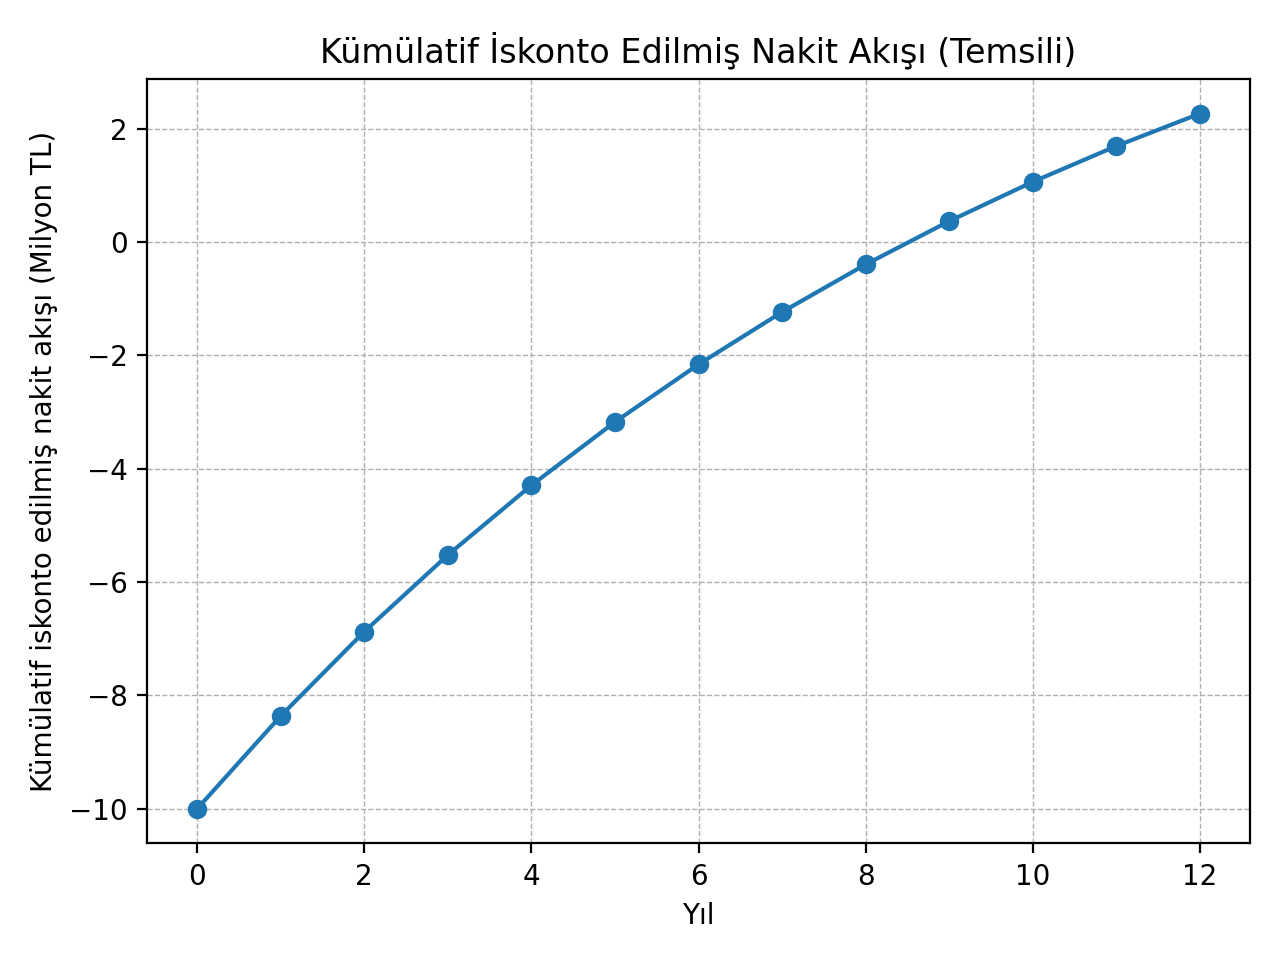
\includegraphics[width=\linewidth]{cum_dcf.png}
\caption{Kümülatif iskonto edilmiş nakit akışı (referans senaryo).}
\end{figure}

\subsection{Duyarlılık (Sensitivity) analizi}
Ödev seviyesinde en kritik iki belirsizlik parametresi:
\begin{enumerate}
\item Elektrik birim fiyatı $p_e$ (TL/kWh)
\item CAPEX birim maliyeti $c_{\text{capex}}$ (USD/kW)
\end{enumerate}
$p_e$ arttıkça yıllık tasarruf ve NPV artar; CAPEX arttıkça NPV azalır.
Gerçek uygulamada enflasyon, tarife yapısı, vergi/teşvikler ve finansman maliyeti de modele eklenmelidir.

\section{Sonuç ve Değerlendirme}
NASA POWER verileri ve 2011 fizibilite raporundan elde edilen tüketim bilgileri birlikte kullanılarak Bartın Limanı için öz tüketim amaçlı PV sistem tasarımı yapılmıştır.
Analizler, yaklaşık $\SI{2.0}{-}\SI{2.5}{MWp}$ bandındaki bir PV sistemin liman için uygulanabilir ve ekonomik bir çözüm sunduğunu göstermektedir.

\begin{thebibliography}{9}
\bibitem{bartin}
Bartın Konteyner Limanı Fizibilite Raporu, Bartın Belediyesi, 2011.
\bibitem{nasa}
NASA Langley Research Center, POWER Data Access Viewer, \url{https://power.larc.nasa.gov/}.
\bibitem{canadian}
Canadian Solar Inc., TOPBiHiKu7 PV Module Datasheet, \url{https://www.canadiansolar.com/}.
\bibitem{irena}
International Renewable Energy Agency (IRENA), Renewable Power Generation Costs, 2024 Report, \url{https://www.irena.org/}.
\end{thebibliography}

\end{document}
